\clearpage
\section{Discussion}

這裏我想討論兩個主題,一個是 accum\-grad 的效果,另一個是 sine linear gamma function 的效果。


\subsection{The effect of accum-grad}

一開始在 review 助教給的 code 的時候,發現這個以前我從來沒有使用過的參數,所以想說來討論一下這個參數的效果。 

\begin{figure}[h]
    \centering
    \begin{subfigure}{0.48\textwidth}
        \centering
        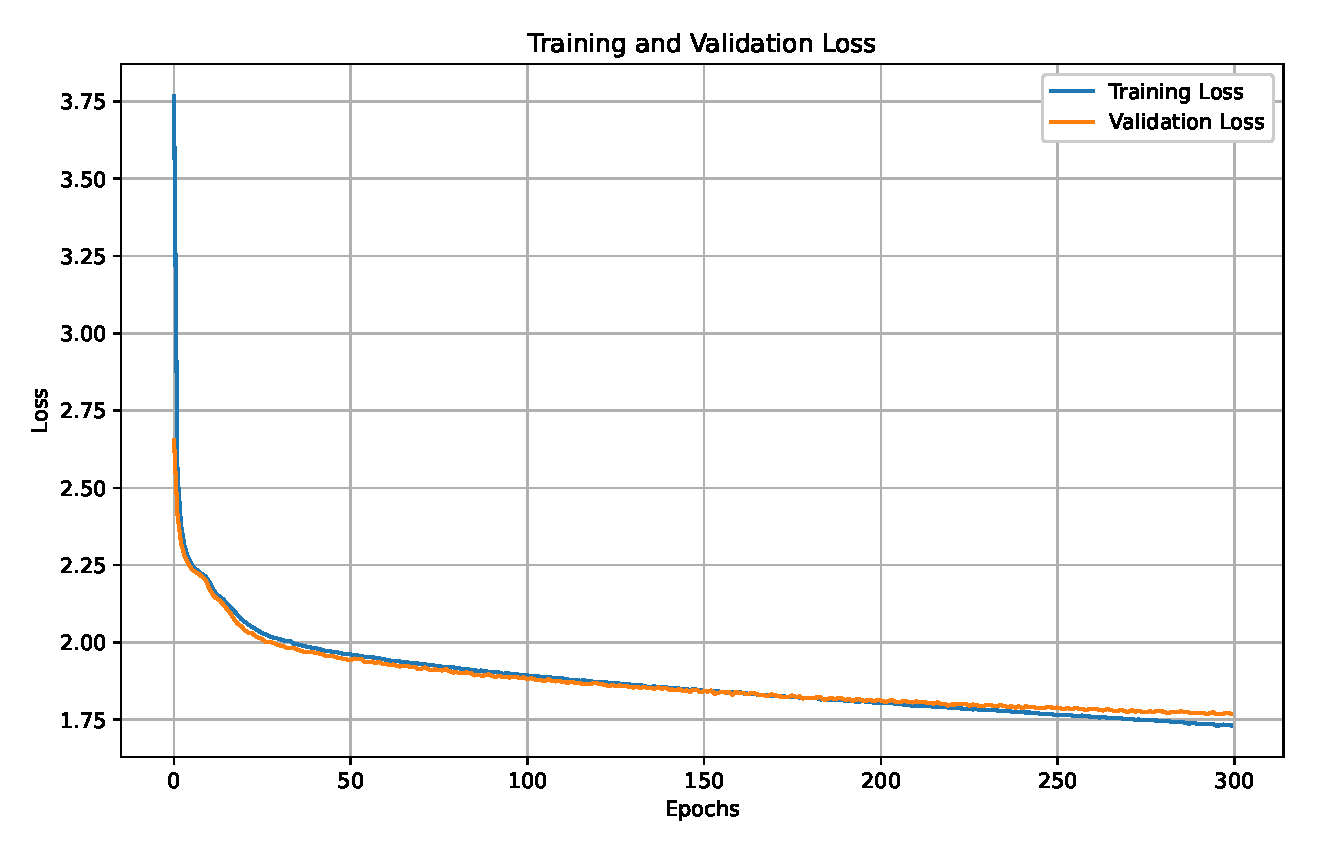
\includegraphics[width=\textwidth]{figures/loss_plot.eps}
        \label{fig:normal_loss_plot}
    \end{subfigure}
    \hfill
    \begin{subfigure}{0.48\textwidth}
        \centering
        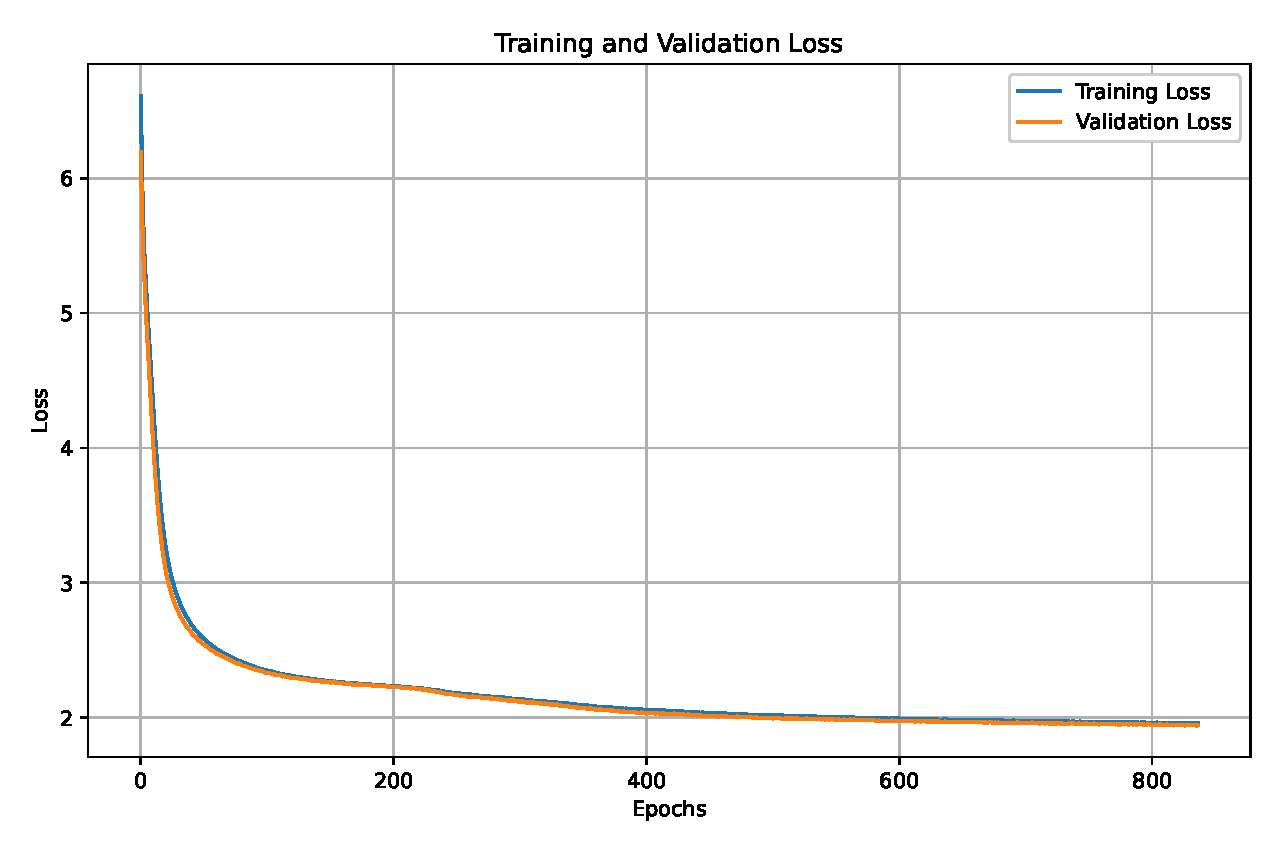
\includegraphics[width=\textwidth]{figures/accum-grad_loss_plot.eps}
        \label{fig:accum-grad_loss_plot}
    \end{subfigure}
    \caption{標準訓練與梯度累積訓練的損失函數對比。左:標準訓練的損失函數;右:梯度累積訓練的損失函數}
    \label{fig:loss_comparison}
\end{figure}




下降的非常慢,而且

\begin{figure}[h]
    \centering
    \begin{subfigure}{0.48\textwidth}
        \centering
        
\includegraphics[width=\textwidth, height=2.1cm, keepaspectratio]{figures/ag-epoch800-test_69.png}
        \label{fig:ag-epoch800-test_69}
    \end{subfigure}
    \hfill
    \begin{subfigure}{0.48\textwidth}
        \centering
        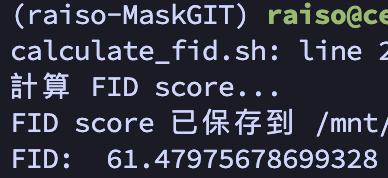
\includegraphics[width=\textwidth, height=2.1cm, keepaspectratio]{figures/ag-fid-score.png}
        \label{fig:ag-fid-score}
    \end{subfigure}
    \caption{梯度累積訓練的測試結果與 FID 分數。左:梯度累積訓練 800 個 epoch 後的測試結果;右:梯度累積訓練的 FID 分數}
    \label{fig:ag-epoch800-test}
\end{figure}




\subsection{The effect of sine linear gamma function}
This is a session of the effect of sine linear gamma function.



\begin{figure}[h]
    \centering
    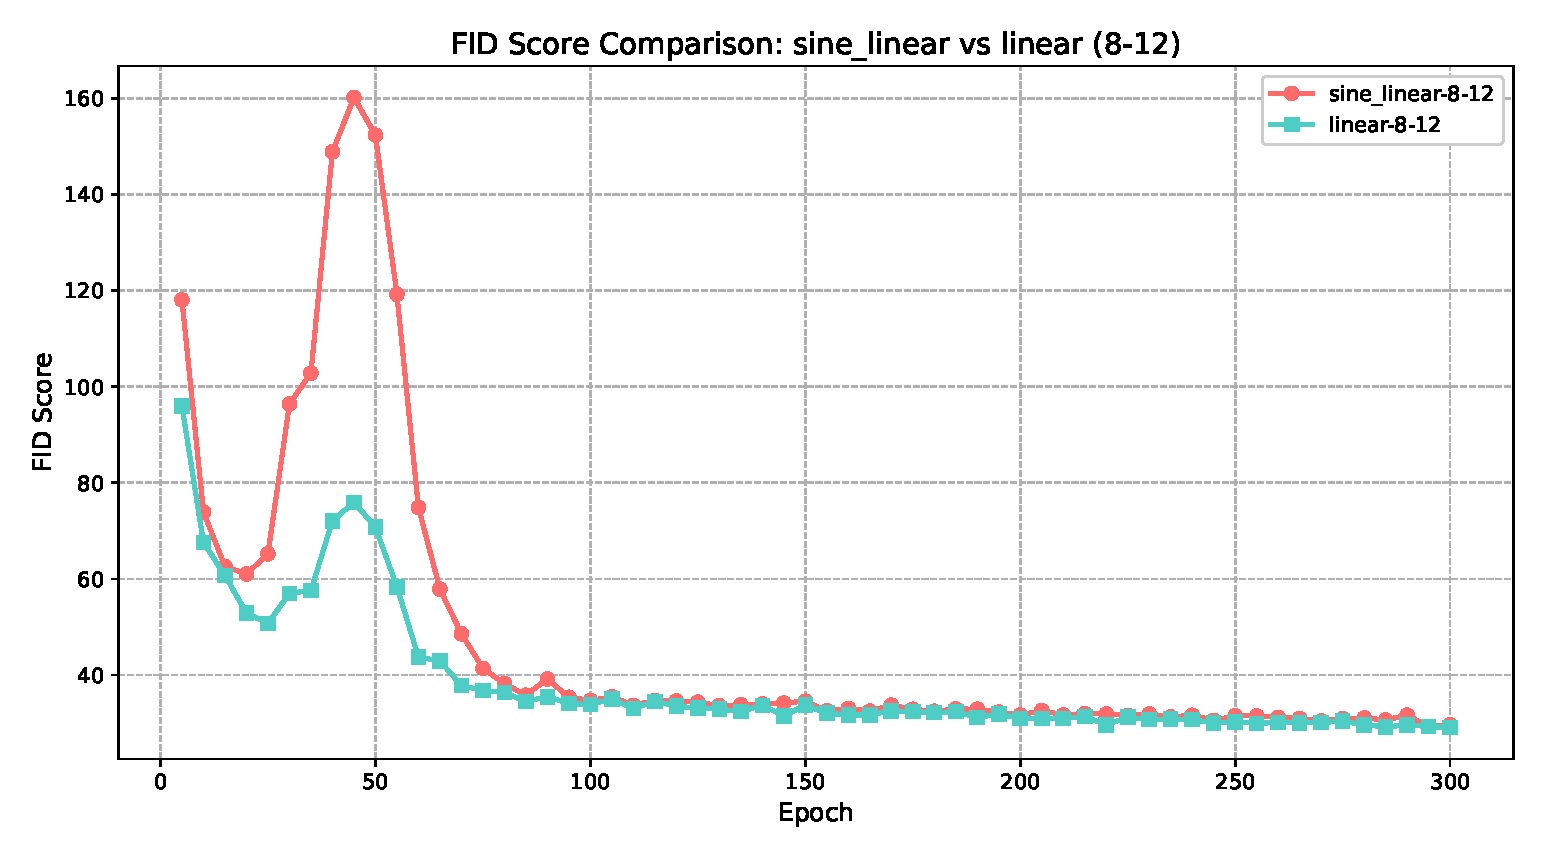
\includegraphics[width=\textwidth]{figures/fid_comparison_8_12.eps}
    \caption{不同 gamma 函數策略的 FID 分數比較}
    \label{fig:fid_comparison_8_12}
\end{figure}


這裡來觀察 fid score 最差的第 45 個 epoch 的結果。

\begin{figure}[h]
    \centering
    \begin{subfigure}{\textwidth}
        \centering
        
\includegraphics[width=0.8\textwidth]{figures/test_69.png}
        \label{fig:mask_test_69}
    \end{subfigure}
    % \vspace{1cm}
    \begin{subfigure}{\textwidth}
        \centering
        
\includegraphics[width=0.8\textwidth]{figures/bad-linear-test_69.png}
        \label{fig:bad-linear-test_69}
    \end{subfigure}
    % \vspace{1cm}
    \begin{subfigure}{\textwidth}
        \centering
        
\includegraphics[width=0.8\textwidth]{figures/bad-sine-linear-test_69.png}
        \label{fig:bad-sine-linear-test_69}
    \end{subfigure}
    \caption{不同 gamma 函數對測試圖像的影響比較。上圖best fid score 的測試圖像;中圖為使用線性 gamma 函數的測試結果;下圖為使用正弦線性 gamma 函數的測試結果}
    \label{fig:gamma-comparison-test}
\end{figure}



可以加入討論計算資源的章節